\documentclass[11pt]{article}

\usepackage{graphicx}
\usepackage{bm}
\usepackage{siunitx}
\usepackage{booktabs}
\usepackage{xcolor}
\usepackage{authblk}
\usepackage{amsmath}
\usepackage{amssymb}
\usepackage{amsthm}
\usepackage{todonotes}
%\usepackage[normalem]{ulem}
\usepackage{float}
\usepackage{commath}
\usepackage{fancybox}
\usepackage{url}
\usepackage[margin=0.5in]{geometry}

\theoremstyle{definition}
\newtheorem{Def}{Definition}[section]
\newtheorem{Eg}{Example}[section]
\newtheorem{Rm}{Remark}[section]
\newtheorem{Ex}{Exercise}[section]
\newtheorem{Prop}[Def]{Proposition}
\newtheorem{Lem}[Def]{Lemma}
\newtheorem{Thm}[Def]{Theorem}
\newtheorem{Cor}[Def]{Corollary}
\newtheorem{Rem}[Def]{Remark}
\newtheorem{Ass}[Def]{Assumption}
\newtheorem{Met}[Def]{Method}
\newtheorem{Res}[Def]{Result}
\newcommand{\red}{\textcolor{red}}
\newcommand{\E}{\mathbb{E}}
\newcommand{\R}{\mathbb{R}}

\usepackage[backend=biber, style=authoryear, citestyle=authoryear, autocite=inline, isbn=true]{biblatex} % package for bibliography 
%\DeclareLanguageMapping{english}{english-apa}

\addbibresource{sdewind.bib}

%\renewbibmacro*{title}{%
%  \ifboolexpr{
%    test {\iffieldundef{title}}
%    and
%    test {\iffieldundef{subtitle}}
%  }
%    {}
%    {\printtext{%
%     \printtext[titlecase]{\usefield{\uline}{title}}%
%     \setunit{\subtitlepunct}%
%     \printfield[titlecase]{subtitle}}%
%     \newunit}%
%  \printfield{titleaddon}}


\newcommand{\add}{\textcolor{red}{[insert]}}

\setcounter{page}{1}

\begin{document}

\title{ Stochastic Wind Power Forecasting }  % \\  \small{Report}}

%\author[1]{Waled Alhaddad}
\author[1]{Renzo Caballero}
\author[2]{Ahmed Kebaier}
\author[3]{Marco Scavino}
\author[4]{ Ra\'ul  Tempone}
%\author[2]{Corresponding Author\thanks{email@2nduniversity.com}}
\affil[1,4]{CEMSE Division, King Abdullah University of Science and Technology (KAUST), Saudi Arabia}
\affil[2]{Université Paris 13, Sorbonne Paris Cité, LAGA, CNRS (UMR 7539), Villetaneuse, France}
\affil[3]{Universidad de la Rep\'ublica, Instituto de Estad\'{\i}stica (IESTA), Montevideo, Uruguay}
\affil[4]{Alexander von Humboldt Professor, RWTH Aachen University, Germany}

%\author{ Waled Alhaddad \textsuperscript{\textasteriskcentered} \qquad Ahmed Kebaier\textsuperscript{\ddag} \qquad Ra\'ul  Tempone\textsuperscript{\textasteriskcentered}\textsuperscript{\textdagger} \\
%\textsuperscript{\textasteriskcentered}CEMSE Division, King Abdullah University of Science and Technology (KAUST), Saudi Arabia \\ \textsuperscript{\textdagger}Alexander von Humboldt Professor, RWTH Aachen University, Germany
% \\ \textsuperscript{\ddag}Université Paris 13, Sorbonne Paris Cité, LAGA, CNRS (UMR 7539), Villetaneuse, France}

\maketitle
%\thispagestyle{empty}

%%%%%%%%% ABSTRACT

\begin{abstract}

Reliable wind power generation forecasting is crucial for applications such as the allocation of energy reserves, optimization of electricity price and operation scheduling of conventional power plant. We propose a data driven model based on parametric Stochastic Differential Equations (SDEs) to captures real-world asymmetric dynamics of wind power forecast errors. Our SDE framework incorporates time derivative tracking of the forecast, time-dependent mean reversion parameter and an improved diffusion term. We are able to simulate future wind power production paths and to get sharp confidence bands. The method is forecast technology agnostic and enables the comparison between different forecasting technologies on the basis of information criteria. We apply the model to historical Uruguayan wind power production data and forecasts on the year 2019.

\end{abstract}

{\color{red}Keywords: Indirect inference, wind power, probabilistic forecasting, stochastic differential equations, Lamperti transform, model selection.}

{\color{red} Add AMS Classification.}

%%%%%%%%% BODY TEXT


%---BEGIN SECTION 1---
\section{Introduction}  \label{Section_1}

\begin{figure}[H]
\centering
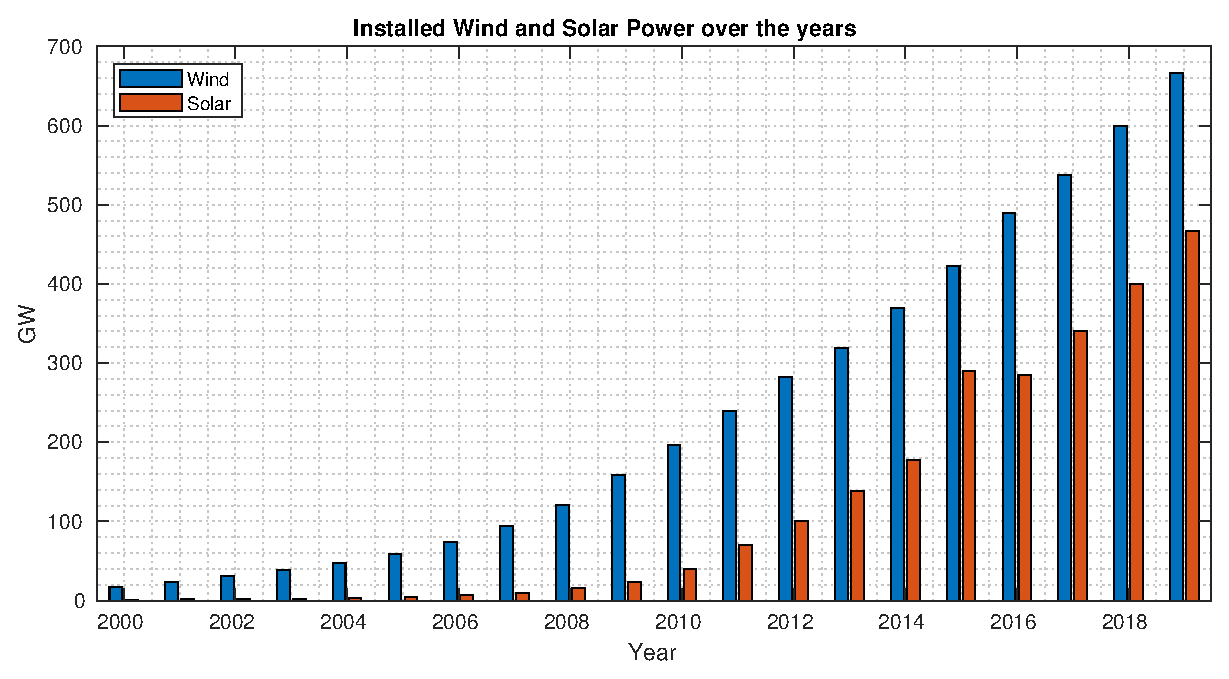
\includegraphics[width=0.9\textwidth]{plots/wind_and_solar/plot_over_years.eps}
\caption{Installed wind and solar power over the years \cite{sultana2017review}. We recall the importance of accurate forecasts to use green energies optimally.}
\end{figure}

Reliable wind power generation forecasting is crucial for the following applications (see, for example, \cite[5]{gieb}, \cite[162]{chang}, \cite{zhbo}):
\begin{itemize}
\item Allocation of energy reserves such as water levels in dams or oil, and gas reserves.
\item Operation scheduling of controlable power plants.
\item Optimization of the price of electricity for different parties such as electric utilities, Transmission system operator (TSOs), Electricity service providers (ESPs), Independent power producers (IPPs), and energy traders.
\item Maintenance planning such as that of power plants components and transmission lines.

\end{itemize}

Different methods have been applied to wind power forecasting. They can be generally categorized as follows: physical models, statistical methods, artificial intelligence methods and hybrid approaches. The output of such methods is usually a deterministic forecast. Occasionally probabilistic forecasts are produced through uncertainty propagation in the data, parameters or through forecast ensembles. {\color{red} Expand discussion about works on probabilistic forecasting.} However, there is a lacking in simulating and producing data driven stochastic forecasts based on real-world performance of forecasting models. It is crucial to capture actual performance of a forecast as it has been known that different forecasting technologies exhibits different behavior for different wind farms and seasons [ref]. This is due to many factors which forecast are challenged to capture such as the surrounding terrains of the wind farm and the condition of the blades such as icing, wear and tear or dirt. It is known that complex terrains in both off shore and on shore locations decrease the accuracy of wind power forecasts significantly [ref]. It also has been shown that the performance of forecasts varies from month to month. Thus the performance of wind power forecasts is location and time dependent.

Many approaches have been taken to evaluate the uncertainty of a given forecast. There are two types of errors: level errors and phase errors. The use of mean or median errors in this context may be misleading as wind power forecast errors are asymmetric. This is a natural consequence of wind power being non-negative and bounded by the maximuim capacity of production. This is important as the associated cost to power forecast errors are also asymmetric due to different costs for up and down  power regulations which are determined by the electricity market [ref].

We propose to model wind power forecasts errors using parametric stochastic differential equations (SDEs) whose solution defines a stochastic process. This resultant stochastic process describes the time evolution dynamics of wind power forecast errors while capturing properties such as a correlation structure and the inherent asymmetry. Additionally, the model we propose is agnostic of the forecasting technology and serves to complement forecasting procedures by providing a data driven stochastic forecast. Hence, we are able to evaluate wind power forecasts according to their real-world performance and we are able to compare different forecasting technologies. Most notably, we are able to simulate future wind power production given a deterministic wind power forecast. Future wind power production using Monte Carlo methods, as well as the analytic form of the proposed SDE, can be used in optimal control problems involving wind power production.

Previous attempt by (\cite{mozuma}) considered stochastic wind power forecast models based on stochastic differential equations. Here, we propose an improved model featuring time derivative tracking of the forecast, time-dependent mean reversion, modified diffusion and non-Gaussian approximations. We apply the model to Uruguayan wind power forecasts together with historical wind power production data pertaining to the year 2019.

{\color{red} REWRITE In this paper we present the phenomenological model based on SDE approach in Section \ref{Section_3} and describe the physical constraints in and how these constrains can be met. Then, in Section \ref{Section_4}, we will introduce an alternative formulation of the model in Lamperti space. In Section \ref{Section_6}, we show our parameter estimation procedure and its results in Section \ref{Section_7}. We compare alternative models in Section \ref{Section_8} and different forecast providers in Section \ref{Section_9}.}

%---END SECTION 1---

%---BEGIN SECTION 2---
\section{Wind power production data in Uruguay and forecast providers } \label{Section_2}

In recent years, Uruguay has triggered a remarkable change in its energy matrix. In (\cite{irena}, p.23) Uruguay is among those countries showcasing innovation, like Denmark, Ireland, Germany, Portugal, and Spain, with proven feasibility of managing annual variable renewable energy higher than 25\% in power systems. 

According to (\cite{ren21}, pp.118-119), in 2018, Uruguay achieved 36\% of its electricity production from variable wind energy and solar PV, raising the share of generation from wind energy more than five-fold in just four years, from 6.2\% in 2014 to 33\% in 2018. 

At present, Uruguay is fostering even higher levels of wind penetration by boosting regional power trading with Argentina and Brazil. 
In this rapidly evolving scenario, it is essential to analyze national data on wind power production joint with wind power short-term forecastings to orientate and assess the strategies and decisions of wind energy actors and businesses. 

Our study is based on publicly available data (source: Administrator of Electric Market) on the wind power production in Uruguay for the period March-December 2019, that we adequately normalized with respect to the present $\SI{1474}{\mega\watt}$ maximum installed wind power capacity. Each day, wind power production recordings are available every ten minutes.  In this work, we have also considered data from three different forecast providers, available each day starting at 1 pm.

The next Figure \ref{fig:sample_data} shows the wind power real production during four segments 24-hour long selected from the observation period together with their corresponding hourly short-term forecast, computed by a forecast provider. For the sake of visualization clarity, this Section relies only on forecasts from one provider, called "provider A" from now on, ranked as the most accurate forecast provider, as it emerged from our posterior analysis. 

\begin{figure}[H]
\centering
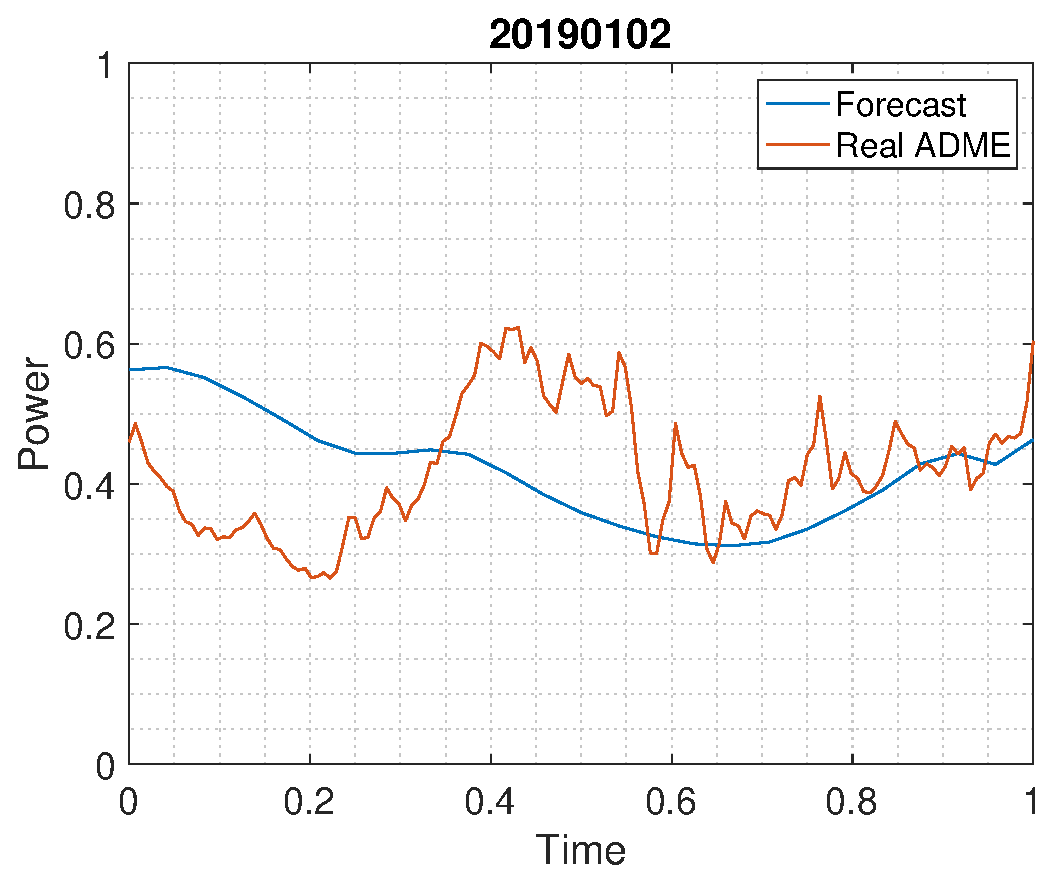
\includegraphics[width=0.35\textwidth]{plots/5.eps}
\includegraphics[width=0.35\textwidth]{plots/245.eps}\\
\includegraphics[width=0.35\textwidth]{plots/661.eps}
\includegraphics[width=0.35\textwidth]{plots/805.eps}
\caption{Four 24-hour segments with the wind power real production in Uruguay (orange line) recorded every ten minutes, and the hourly wind power production forecasted by provider A (blu line).}
  \label{fig:sample_data}
\end{figure}

A global view of the discrepancy between the real production and the forecasted production, the forecast error, during the nine months observation period, is displayed in the following Figure \ref{fig:data_curtailing}, where we also partitioned the forecast errors according to three contiguous categories of normalized generated power. Low normalized generated power corresponds to the range $[0,0.3]$, mid-power refers to the range $(0.3,0.6]$, and high-power to the range $(0.6,1]$.

\begin{figure}[H]
\centering
\includegraphics[width=0.35\textwidth]{plots/LP_6.eps}
\includegraphics[width=0.35\textwidth]{plots/MP_6.eps}\\
\includegraphics[width=0.35\textwidth]{plots/HP_6.eps}
\includegraphics[width=0.35\textwidth]{plots/AP_6.eps}
\caption{Wind production forecast error histograms during the period March-December 2019: low-power (upper-left graph), mid-power (upper-right graph), high-power (lower-left graph), and the global range of power (lower-right graph).}
  \label{fig:data_curtailing}
\end{figure}

We may observe that all the histograms in the Figure \ref{fig:data_curtailing} exhibit skewed patterns, to a different extent, as well as extreme observations. The presence of these features can be partly explained. The analysis of the dataset highlighted that, during several 24-hour segments, the system operators decided to reduce, or even cease the wind power production {\color{red} add why curtailment and references}. 

The curtailment of the wind power production imposed by the system operators has a strong influence on the forecast error. To build a model that, driven by the available forecast, allows to include the true power production with a prescribed degree of uncertainty, it is necessary to remove the data segments affected by wind curtailment.

Once we removed all the 24-hour segments associated with wind curtailment, we kept 147 segments. In the absence of the curtailment effect, the forecast error histograms are shown in Figure \ref{fig:data_after_clean} below, where it is appreciable the reduction of skewness.

\begin{figure}[H]
\centering
\includegraphics[width=0.35\textwidth]{plots/LP.eps}
\includegraphics[width=0.35\textwidth]{plots/MP.eps}\\
\includegraphics[width=0.35\textwidth]{plots/HP.eps}
\includegraphics[width=0.35\textwidth]{plots/AP.eps}
\caption{Wind production forecast error histograms during the period March-December 2019 after removing 24-hour segments with artificial wind curtailment: low-power (upper-left graph), mid-power (upper-right graph), high-power (lower-left graph), and the global range of power (lower-right graph).}
  \label{fig:data_after_clean}
\end{figure}

In this stage of data preprocessing, we obtain another useful result by applying the first-order difference operator to the forecast errors. 
The forecast error transition histograms, displayed in the next Figure \ref{fig:error_transitions}, will constitute later a reference for the visual assessment of the global fit of the proposed models.

\begin{figure}[H]
\centering
\includegraphics[width=0.35\textwidth]{plots/LP_t.eps}
\includegraphics[width=0.35\textwidth]{plots/MP_t.eps}\\
\includegraphics[width=0.35\textwidth]{plots/HP_t.eps}
\includegraphics[width=0.35\textwidth]{plots/AP_t.eps}
\caption{Forecast error transition histograms during the period March-December 2019 without wind power production curtailment: low-power (upper-left graph), mid-power (upper-right graph), high-power (lower-left graph), and the global range of power (lower-right graph).}
\label{fig:error_transitions}
\end{figure}

 {\color{red}  We can observe the lack of gaussianity.}

 ({\color{red} MOVE THIS COMMENT. We use 73 days to train the system and 74 to test it. Also, to avoid correlation between days, we intercalate the days we use for training and testing. Show that 24h is enough to ensure independence}).


%---END SECTION 2---

%---BEGIN SECTION 3---
\section{Phenomenological  Model} \label{Section_3}

After analyzing the available dataset, we are now in the condition to build a type of phenomenological model for the normalized wind power generation forecasts that, in its most general form, is a stochastic process $X = \{X_t, \, t \in [0, T] \}$  defined by the following stochastic differential equation (SDE):

\begin{equation}
  \left\{
  \begin{array}{@{}rl@{}}
    dX_t \!\!\!&=  a(X_t; p_t, \dot{p}_t,\bm{\theta}) \,dt + b (X_t; p_t, \dot{p}_t, \bm{\theta} ) \,dW_t\,, \quad t \in [0,T]  \\
     X_0  \!\!\!&=  x_0 \in [0,1],
  \end{array}\right. \label{eq:main}
\end{equation} 

where

\begin{itemize}
\item $a(\cdot; p_t, \dot{p}_t, \bm{\theta}): [0,1] \to \mathbb{R} $  denotes a drift function,
\item $b(\cdot; p_t, \dot{p}_t, \bm{\theta}): [0,1] \to \mathbb{R}_+ $  a  diffusion function,
\item $\bm{\theta}$ is a vector of unknown parameters,
\item $(p_t)_{t \in [0,T]}$ is a time-dependent deterministic function $[0,1]$-valued and $ (\dot{p}_t)_{t \in [0,T]}$ is its time derivative,
\item $\{W_t, \, t \in [0,T] \}$ is a standard real-valued Wiener process.
\end{itemize}

In this work, $(p_t)_{t \in [0,T]}$ is to be considered as a deterministic forecast for the normalized wind power generation, which is provided by an official source. 

Our goal is to achieve a specification of the model (\ref{eq:main}) to follow closely the available normalized wind power forecasts while ensuring its unbiasedness with respect to the forecast. 

\subsection{Physical Constraints} \label{Physical_Constraints}

Let $(p_t)_{t \in [0,T]}$ be the available prediction function for the normalized wind power, which is an input to this approach. To start with the model specification, first we introduce a time-dependent drift function that features the mean-reverting property as well as derivative tracking:
\begin{equation}
a(X_t; p_t, \dot{p}_t, \bm{\theta}) = \dot{p}_t  - \theta_t (X_t - p_t)\,,  \label{drift:meanrev-derivtrack}
\end{equation} 
where $ (\theta_t)_{t \in [0,T]} $ is a positive deterministic function, whose range depends on $\bm{\theta}$, as will be explained shortly.

Now, looking at the normalized wind power generation forecast process $X$, modeled as solution to the It\^{o} stochastic differential equation (\ref{eq:main}) with the drift specified in (\ref{drift:meanrev-derivtrack}), it is straightforward to check that $\mathbb{E} X_t = p_t$, given $  \mathbb{E} X_0 = p_0$. The application of  It\^{o}'s lemma on $g(X_t, t) = X_t e^{\int_{0}^{t} \theta_s ds}$, leads to 
\begin{equation*}
d \left( X_t e^{\int_{0}^{t} \theta_s ds} \right) = e^{\int_{0}^{t} \theta_s ds} (\dot{p}_t + \theta_t p_t ) dt  + e^{\int_{0}^{t} \theta_s ds}\, b (X_t; p_t, \dot{p}_t, \bm{\theta} ) \,dW_t\,,
\end{equation*}
whose integral form is
\begin{equation}
e^{\int_{0}^{t} \theta_s ds}  X_t - X_0 = \int_{0}^{t}  (\dot{p}_s + \theta_s p_s ) e^{\int_{0}^{s} \theta_u du} ds + \int_{0}^{t}  b (X_s; p_s, \dot{p}_s, \bm{\theta} )  e^{\int_{0}^{s} \theta_u du}\, d W_s\,.   \label{eq:tomeanX}
\end{equation} 
Taking expectation on (\ref{eq:tomeanX}) we obtain
\begin{align}
\mathbb{E} X_t & = e^{ - \int_{0}^{t} \theta_s ds} \left(  \mathbb{E} X_0 +   \int_{0}^{t}  (\dot{p}_s + \theta_s p_s ) e^{\int_{0}^{s} \theta_u du} ds   \right) \nonumber \\ 
& =  e^{ - \int_{0}^{t} \theta_s ds} \left(  \mathbb{E} X_0 +   \int_{0}^{t}  \dot{p}_s e^{\int_{0}^{s} \theta_u du} ds +  \big[ p_s \, e^{\int_{0}^{s} \theta_u du} \big]^{t}_0  - \int_{0}^{t}  \dot{p}_s e^{\int_{0}^{s} \theta_u du} ds  \right) \nonumber \\
& =  e^{ - \int_{0}^{t} \theta_s ds} \left(  \mathbb{E} X_0 + p_t \, e^{ \int_{0}^{t} \theta_s ds} - p_0 \right) = p_t \,. \label{eq:meanX}
\end{align}

 At this stage, the process defined by (\ref{eq:main}) with drift (\ref{drift:meanrev-derivtrack}) satisfies the two following properties: 
\begin{itemize}
\item it reverts to its mean $p_t$, with a time-varying speed $ \theta_t$ that is proportional to the deviation of the process $X$ from its mean,
\item it tracks the time derivative $\dot{p}_t$.  
\end{itemize} 

Remark: Observe that a mean-reverting model without derivative tracking shows a delayed path behavior. For instance, consider the diffusion model (\ref{eq:main}) with $a(X_t; p_t, \bm{\theta}) = - \theta_0 (X_t - p_t)\,, \theta_0 > 0$. In this case, given  $ \mathbb{E} X_0 = p_0$, the diffusion has mean $\mathbb{E} X_t = p_t - e^{- \theta_0 t } \int_0^t \dot{p}_s  e^{\theta_0 s} ds$. The next Figure (\ref{fig:derivative_tracking}) illustrates paths of two diffusions with and without derivative tracking. 

\begin{figure}[h]
  %\includegraphics[width=26mm,scale=1]{}
  \caption{{\color{red} Add Figure showing the difference with and without derivative tracking}}
  \label{fig:derivative_tracking}
\end{figure}

The forecast and production wind power data of Uruguay are normalized with respect to the installed power capacity during the period of observation. Thus, the mean-reverting level lies in $[0,1]$, and the process $X$  must take values in the same interval, a requirement that is not automatically fulfilled through the derivative tracking. To impose that the state space of $X$ is $[0,1]$, we may choose a convenient diffusion term, and require that the time-varying parameter $ \theta_t$ satisfies an ad-hoc condition.
 
Let $\bm{\theta} = (\theta_0,\alpha)$, and choose a state-dependent diffusion term that avoids the process exiting from the range $[0,1]$ as follows:
  \begin{equation}
    b (X_t; \bm{\theta} )= \sqrt{2 \alpha \theta_0 X_t (1 - X_t)}
  \end{equation}
  where $\alpha >0$ is a unknown parameter that controls the path variability. This diffusion term belongs to the Pearson diffusion family and, in particular, it defines a Jacobi type diffusion. It is useful to recall that (\cite[440]{foso}) a Pearson diffusion is a stationary solution to a stochastic differential equation of the form
 \begin{equation}
    dX_t = - \theta (X_t - \mu) dt + \sqrt{2 \theta (a X_t^2 + b X_t + c)} dW_t
  \end{equation}
where $\theta>0$, and $a$, $b$ and $c$ are parameters such that the square root is well defined when $X_t$ is in the state space. These parameters, together with $\mu$, the mean of the invariant distribution, determine the state space of the diffusion as well as the shape of the invariant distribution. 

An exhaustive classification of the (stationary) Pearson diffusions is presented in (\cite[440-443]{foso}) where, in particular, it is discussed the case $a < 0$ and $b(x; \bm{\theta}) = \sqrt{2 a \theta x (x-1)}$, where the invariant distribution is a Beta distribution with parameters $\left( \frac{\mu}{-a}, \frac{1 - \mu}{-a} \right),$ that leads to the well-known Jacobi diffusions, so-called because the eigenfunctions of the infinitesimal generator of these processes are the Jacobi polynomials (see, for example, \cite[2860-2861]{leph}). 

It is worth mentioning that Jacobi diffusions have been successfully applied in several disciplines, among them finance (see \cite{vago} and references therein) and neuroscience (\cite{dotala}).

However, a distinctive feature in our proposed model 
\begin{equation}
  \left\{
  \begin{array}{@{}rl@{}}
    dX_t \!\!\!&= (\dot{p}_t  - \theta_t (X_t - p_t) ) dt +\sqrt{2 \alpha \theta_0 X_t (1 - X_t)} dW_t\,, \quad t \in [0,T]  \\
   X_0  \!\!\!&=  x_0\in [0,1] \,,
 \end{array}\right.  \label{ourmodel}
\end{equation}

is that the drift term contains the time-varying parameter $\theta_t$, rendering the solution $X$ to (\ref{ourmodel}) a non-stationary and time-inhomogeneous process. To ensure that the process $X$ be the unique strong solution to (\ref{ourmodel}) for all $t \in [0,T]$ with state space $[0,1]$ a.s., the mean-reversion time-varying parameter must satisfy the following condition:
%has to be selected according to the following rule. Observe that the time derivative term $\dot{p}_t $ is not controlled to maintain that $X_t$ stays a.s. inside the range $[0,1]$. In other words, the zero drift line defined by $a(x; p_t,\bm{\theta}) =0$, which is an attractor, must be contained inside the range $[0,1]$. Thus, we must have that
%\begin{equation}
%\frac{- |\dot{p_t}|}{p_t} \leq \theta_t \leq \frac{|\dot{p}_t|}{1- p_t}
%\end{equation}
%which is satisfied  by choosing a time-dependent  $\theta_t$ as follows,
%\begin{equation}
%\theta_t = \max \left( \theta_0 \ , \ \frac{|\dot{p}_t|}{\min (p_t, 1-p_t)}  \right ),  \quad \theta_0 >0\,. \label{theta_t}
%\end{equation}
\begin{equation}\label{Assumption:3}
\theta_t\geq \max\left(\frac{\alpha\theta_0+\dot p_t}{1-p_t},\frac{\alpha\theta_0-\dot p_t}{p_t}\right)\tag{B}. 
\end{equation} \label{condB}
The proof of this theoretical statement is presented in Section \ref{Appendix}. \\

Remark: Condition (B) shows that the time-varying parameter $\theta_t$ becomes unbounded when $p_t = 0$ or $p_t = 1$. Therefore, we consider the following truncated prediction function
\begin{equation}
  p_t^{\epsilon} = \left\{
  \begin{array}{@{}cl@{}}
    \epsilon \!\!\!&\text{if \quad} p_t  < \epsilon  \\
    p_t  \!\!\!&\text{if \quad}  \epsilon \leq p_t < 1 - \epsilon \\
    1 - \epsilon  \!\!\!&\text{if \quad}  p_t \geq 1 - \epsilon
 \end{array}\right.  \label{corrforecast}
\end{equation}
that satisfies $p_t^{\epsilon} \in [\epsilon, 1 - \epsilon]$ for any $0 < \epsilon < \frac{1}{2}$ and $t \in [0,T]$, providing that $\theta_t$ is bounded for every $t \in [0,T]$. \\
From now on, we will keep the notation $p_t$ to denote the truncated prediction function (\ref{corrforecast}), unless specified otherwise.

%{\color{red} The expression for $\theta_t$ is important: $\theta_t$ depens on $t$ through $\dot{p_t}$ and $p_t$. Besides it is parsimonious because only one unknown parameter appear in \ref{theta_t}. Recall it is an upped bound for the real inequality. } 


%\subsubsection*{Change of Variables:}
\subsection{A model specification for the forecast error}
 After applying to (\ref{ourmodel}) the simple change of variables $$V_t = X_t - p_t \,,$$ we may introduce the following model for the forecast error of the normalized wind power production: 

\begin{equation}
  \left\{
  \begin{array}{@{}rl@{}}
    dV_t \!\!\!&=  - \theta_t V_t  \, dt + \sqrt{2 \alpha \theta_0 (V_t +p_t ) (1-V_t-p_t)} \, dW_t\,, \quad t \in [0,T]  \\
   V_0  \!\!\!&=  v_0\in [-1 + \epsilon,1 - \epsilon] \,.
 \end{array}\right.  \label{VtSDE}
\end{equation}


%---END SECTION 3---


%---BEGIN SECTION 4---
\section{State independent diffusion term: Lamperti transform} \label{Section_4}

Our model (\ref{VtSDE}) for the forecast error has a diffusion term that depends on the state variable $V_t$. To estimate the unknown model parameters, a recommended technique is to modify the SDE (\ref{VtSDE}) by applying the so-called Lamperti transform (see \cite[40--41]{iacus1}, \cite{moma}, \cite[98--100]{saso}) to the process $V$ to obtain a SDE for the transformed process whose diffusion term does not depend anymore on the state variable. To this purpose, we consider the following Lamperti transformation  
%{\color{red} (Remind that continuous-time models with different diffusion term are singular and the likelihood cannot be written down. Besides, it can be unstable to work with low frequency. If the frequency of the data is too low, the Lamperti transform helps to detect this problem (in principle, it is not clear how to determine the right frequency for estimation. )}
%\begin{equation}
%Z_t = h(V_t, t) = \frac{1}{\sqrt{2 \theta_0 \alpha}} \int_{\xi}^{x} \frac{1}{\sqrt{(u + p_t)(1 - u - p_t)}} \,du \Bigg{\vert}_{x = V_t} \,,
%\end{equation}
%where $\xi$ is an arbitrary point of the state space of the process $V$. The choice of $\xi = \frac{1}{2} - p_t$, where $p_t$ is a known input, 
\begin{align}
Z_t = h(V_t, t; \bm{\theta} )  & = \frac{1}{\sqrt{2 \alpha \theta_0 }} \int \frac{1}{\sqrt{(v + p_t)(1 - v - p_t)}} \,dv \Bigg{\vert}_{v = V_t}   = - \sqrt{ \frac{2}{ \alpha \theta_0 }} \arcsin (\sqrt{ 1 - V_t - p_t}) \label{eq:LampZ}
\end{align}
that, after applying It\^{o}'s formula on $h(V_t, t)$, leads to the following SDE with state independent unit diffusion term
\begin{align}
dZ_t = \Bigg[  & \frac{\dot{p}_t}{ \sqrt{2 \alpha \theta_0 (V_t + p_t)(1 - V_t - p_t)}}  + \frac{- \theta_t V_t}{ \sqrt{2  \alpha \theta_0 (V_t + p_t)(1 - V_t - p_t)}} - \frac{1}{4} \frac{\sqrt{2 \alpha \theta_0} \left( 1 - 2 (V_t + p_t)\right)}{\sqrt{(V_t + p_t)(1 - V_t - p_t)}}  \Bigg] \,dt + dW_t \,. \label{eq:stindepSDE}
\end{align}
After replacing $V_t = 1 - p_t - \sin^2 \left(- \sqrt{ \frac{ \alpha \theta_0}{2} } Z_t \right) $ in (\ref{eq:stindepSDE}), we obtain that the  process $Z$ satisfies the SDE
\begin{align}
dZ_t & = \Bigg[ \frac{ \dot{p}_t  - \theta_t  \left(1 - p_t - \sin^2 \Big(- \sqrt{ \frac{ \alpha \theta_0}{2} } Z_t \Big) \right) }{\sqrt{2 \alpha \theta_0} \cos\Big(- \sqrt{ \frac{ \alpha \theta_0}{2} } Z_t \Big)  \sin\Big(- \sqrt{ \frac{ \alpha \theta_0}{2} } Z_t \Big)}   - \frac{1}{4}  \frac{\sqrt{2 \alpha \theta_0} \left(1 - 2 \cos^2 \Big(- \sqrt{ \frac{ \alpha \theta_0}{2} } Z_t \Big) \right) }{\cos\Big(- \sqrt{ \frac{ \alpha \theta_0}{2} } Z_t \Big)  \sin\Big(- \sqrt{ \frac{ \alpha \theta_0}{2} } Z_t \Big)} \Bigg] \,dt + dW_t \nonumber \\
&  = \left[  \frac{  2  \dot{p}_t - \theta_t (1 - 2 p_t)  + (\alpha \theta_0 - \theta_t) \cos(- \sqrt{2 \alpha \theta_0 } Z_t) }{\sqrt{2 \alpha \theta_0} \sin{(- \sqrt{2 \alpha \theta_0} Z_t)}}  \right] \,dt + dW_t \,.  \label{eq:stindepSDE2}
\end{align}

{\color{red} We can see in Figure (\ref{fig:LP_transitions}) the effect of the Lamperti transformation upon the forecast error data. 

\begin{figure}[H]
\centering
\includegraphics[width=0.35\textwidth]{plots/LP_t_LP.eps}
\includegraphics[width=0.35\textwidth]{plots/MP_t_LP.eps}\\
\includegraphics[width=0.35\textwidth]{plots/HP_t_LP.eps}
\includegraphics[width=0.35\textwidth]{plots/AP_t_LP.eps}
\caption{Transitions after the Lamperti transform. The transitions now present a normal Gaussian shape. This effect motivates the use of Gaussian proxies to approximate the process after using the Lamperti transform.}
  \label{fig:LP_transitions}
\end{figure}

The Lamperti transformation has greatly reduced the forecast error skewness, ensuring that the process stays in the range $[0,1]$. Therefore, in this case, the transition densities of the process Z can be adequately approximated through Gaussian densities.}

%{\color{red} Remind that Lamperti transform has the purpose tho check the consistency of the models, that is if the estimation of $\bm{\theta}$ with $V$ and $Z$ differs it is alarming.}

%---END SECTION 4---

%---BEGIN SECTION 5---
\section{ Likelihood functions of the forecast errors data and optimization algorithm} \label{Section_5} 

\subsection{Likelihood in the $V-$space}

Suppose that any of $M$ non-overlapping paths of the continuous-time It\^{o} process $V = \{ V_t, t  \in [0,T] \}$ is sampled at $N + 1$ equispaced discrete points with given length interval $\Delta$, and let $ V^{M,N + 1}=\{ V_{t_1^{N + 1}} , V_{t_2^{N + 1}} ,\ldots , V_{t_M^{N + 1}} \}$ denote this random sample, with $V_{t_j^{N + 1}} = \{ V_{t_j + i \Delta}\,, i = 0, \ldots, N \}, \, j = 1, \ldots, M$. 

Let $\rho(v \vert v_{j, i-1} ; \bm{\theta})$ be the conditional probability density of $V_{t_j + i \Delta} \equiv V_{j, i}$ given $V_{j, i-1} = v_{j, i-1}$ evaluated at $v$, where $\bm{\theta} = (\theta_0, \alpha, \epsilon)$ are the unknown model parameters.

The It\^{o} process $V$ defined by the SDE (\ref{VtSDE}) is Markovian, then the likelihood function of the sample $ V^{M,N + 1}$ can be written as the following product of transition densities:  

\begin{equation}
\mathcal{L}(\bm{\theta}; V^{M,N +1}) = \prod\limits_{j=1}^M \left\{ \prod\limits_{i=1}^N \rho ( {V_{j, i}| V_{j, i-1}} ; p_{[t_{j,  i-1}, t_{j , i} ]},  \bm{\theta} )  \,  \right\} \,,
\label{likelihood}
\end{equation}
where $t_{j ,i} \equiv  t_j + i \Delta$ for any $j = 1, \ldots, M$ and $i = 0, \ldots, N$.

 {\color{red} Remark: The statistical model (\ref{likelihood}) can be generalized incorporating the transition that occurs during the time interval, say $\delta$, between the time when the forecast is done and the first date of forecasting. In this case, the inner product in  (\ref{likelihood}) must include for any of the $M$ paths an additional factor, say $\rho_0 (V_{j, 0}|V_{j, -\delta};\bm{\theta},\delta)$, expressing the conditional density of this early transition. The parameter $\delta$ can be calibrated after the estimation of $\bm{\theta}$, suggesting an optimal time for the scheduling of the forecasts.}

The exact computation of the likelihood (\ref{likelihood}) relies on the availability of a closed-form expression for the transition densities of $V$ that, on the basis of the Markovian property of $V$, are characterized, for $ t_{j, i-1} < t < t_{j,i}$,  as solutions of the Fokker-Planck-Kolmogorov equation (\cite[36]{iacus1}, \cite[61-68]{saso}):

\begin{align}
\frac{ \partial f }{\partial t } & \rho(v ,t \vert v_{j,i-1} ,  t_{j,i-1} ; \bm{\theta} )= - \frac{\partial}{ \partial v} (- \theta_t v \, \rho(v ,t \vert v_{j,i-1} ,  t_{j,i-1} ; \bm{\theta} ) ) \nonumber \\
& + \frac{1}{2} \frac{\partial^2}{ \partial v^2} ( 2 \theta_0 \alpha (v+ p_t) (1 - v- p_t) \, \rho(v ,t \vert v_{j,i-1} ,  t_{j,i-1} ; \bm{\theta} ) )\,,  \label{eq:fpk}
\end{align}
subject to the initial conditions $\rho(v , t_{j, i-1} ; \bm{\theta} ) = \delta(v - V_{j, i-1}) \,,$ where $ \delta(v - V_{j, i-1})$ is the Dirac-delta generalized function centered at $ V_{j, i-1}\,.$

Closed-form solutions to initial-boundary value problem for time-in\-ho\-mo\-geneous diffusions can be obtained only in a few cases (see, for example, \autocite[Section 3.1]{eglix}). Besides, in our case solving numerically (\ref{eq:fpk}) for the transition densities of the process $V$ at every transition step is computationally expensive. 
Therefore, under the likelihood-based inferential paradigma, many techniques have been devised to obtain approximate maximum likelihood estimates for the unknown parameters of continuous-time SDE models with discrete observations. 
 {\color{red} Rewrite: Parametric estimation problems for diffusion processes sampled at discrete times are presented in \autocite[Chapter 3]{iacus1}, consider Preston and Wood, then Egorov, and then Sorensen, remove the
 survey of estimation methods for the parameter vector of the general one-dimensional, time-homogeneous SDE from a single sample of observations at discrete times is presented in \autocite{hurn}, refer to time-homogeneous.}

\subsection{Approximate likelihood  in the $V-$space}

Gaussian approximations to the transition densities of nonlinear time-in\-ho\-mo\-geneous SDEs are available through different algorithms  \autocite[Chapter 9]{saso}. However, as Figure \ref{fig:error_transitions} may suggest at a first glance, the choice of a Gaussian density could be inadequate when straightly applied to approximate the transition density of the forecast error $V$ of the normalized wind power production. 

Therefore, we propose to use a surrogate transition density for $V$ other than Gaussian. The moments of the SDE model (\ref{VtSDE}) are then matched to the moments of the surrogate density. 

From (\ref{eq:meanX}), we have $m_1(t) \equiv \mathbb{E} V_t = e^{- \int_{t_{j,i-1}}^t \theta_s ds} \,\mathbb{E} V_{t_{j,i-1}}$, for any $t\in [t_{j,i-1}, t_{j, i})$, $j = 1, \ldots, M$ and $i = 1, \ldots, N$ .

For $m \geq 2$, using It\^o's lemma on $g(V_t) = V_t^m$, we obtain
% arrive at the following iterative ODEs for the state dependent diffusion formulation (\ref{VtSDE})
\begin{align}
d(V_t^m) & = \left( - m \theta_t V_t^m + \frac{1}{2} m (m -1) V_t^{m -2} 2 \alpha \theta_0 (V_t + p_t) (1 - V_t - p_t) \right) dt  \nonumber \\
& + m V_t^{m-1} 2 \alpha \theta_0 (V_t + p_t) (1 - V_t - p_t) dW_t \,, \nonumber
\end{align}
from which we derive
\begin{equation}
\frac{d \mathbb{E}[ V^m_t]}{dt} = - m \theta_t \mathbb{E}[ V^m_t] + m (m-1) \alpha \theta_0  \mathbb{E}[ - V_t^m + (1 - 2 p_t) V_t^{m-1} + p_t (1 -p_t) V_t^{m-2} ] \,.
\end{equation}

For any $t\in [t_{j,i-1}, t_{j, i})$, the first two moments of $V$, $m_1(t)$ and $m_2(t) \equiv \mathbb{E}[V_t^2]$, can be computed by solving the following system
\begin{equation}
  \left\{
  \begin{array}{@{}rl@{}}
    \frac{d m_1 (t)}{dt} \!\!\!&=  - m_1(t)\theta_t   \\
   \frac{d m_2 (t)}{dt}  \!\!\!&=  -2 (\theta_t +\alpha \theta_0) m_2(t) + 2 \alpha\theta_0 (1-2p_t)  m_1(t) + 2 \alpha\theta_0 p_t (1-p_t) 
 \end{array}\right.  \label{Vtmom}
\end{equation}
with initial conditions $m_1(t_{j,i-1})= v_{j, i-1}$ and $m_2(t_{j,i-1})= v_{j, i-1}^2 \,.$


\subsubsection*{ Moment Matching}
A suitable candidate for a surrogate transition density of $V$ is a Beta distribution on a compact interval parameterized by two positive shape real parameters, $\xi_1, \xi_2$. 

To approximate the transition densities of  the process $V$ using a Beta distribution, we equal the first two central moments of $V$ with the corresponding moments of the Beta surrogate distribution on $[-1 + \epsilon,1 - \epsilon]$ with shape parameters $\xi_1, \xi_2$ . 

The shape parameters are given by
\begin{equation}
\xi_1 = - \frac{(\mu_t + 1 - \epsilon)(\mu_t^2 + \sigma_t^2 - (1- \epsilon)^2)}{2 (1 - \epsilon) \sigma_t^2}\,, \quad \xi_2=  \frac{(\mu_t-1 + \epsilon )(\mu_t^2 + \sigma_t^2 - (1- \epsilon)^2)}{2 (1 - \epsilon) \sigma_t^2} \,, \label{param_transformed_beta}
\end{equation}
where $\mu_t = m_1 (t)$ and $\sigma_t^2= m_2 (t)- m_1 (t)^2\,.$ \\

The approximate log-likelihood $\tilde{\ell}(\cdot ; v^{V, N+1})$ of the observed sample $v^{V, N+1}$ can be expressed as 
\begin{equation}
 \tilde{\ell} (\bm{\theta}; v^{M,N +1}) = \sum_{j=1}^M \sum_{i=1}^N \log  \left\{ \frac{1}{2(1 - \epsilon)} \frac{1}{B(\xi_1, \xi_2)} \Big( \frac{z_{j,i} + 1 - \epsilon}{2(1 - \epsilon)} \Big)^{\xi_1 -1}  \Big( \frac{1 - \epsilon - z_{j,i}}{2(1 - \epsilon)} \Big)^{\xi_2 -1} \right\} \,,
\label{loglikelihoodV}
\end{equation}
where the shape parameters $\xi_1$ and $\xi_2$, according to (\ref{param_transformed_beta}), depend on the quantities $\mu(t_{j,i};\bm{\theta} )$ and $\sigma^2(t_{j,i};\bm{\theta} )$ that are computed solving numerically the initial-value problem (\ref{Vtmom}). \\


\subsection{Approximate likelihood  in the $Z-$space}

The transition density of the process $Z$, which has been defined through the Lamperti transformation (\ref{eq:LampZ}) of $V$, can be conveniently approximated by a Gaussian surrogate density. 

The drift coefficient $a(Z_t; p_t, \dot{p}_t, \bm{\theta}) $ of the process $Z$ that satisfies (\ref{eq:stindepSDE2}) is nonlinear. After linearizing the drift around the mean of $Z$, $\mu_Z(t) \equiv \mathbb{E}Z_t$,  we obtain the following system of ODEs to compute, for any $t\in [t_{j,i-1}, t_{j, i})$, the approximations of the first two central moments of $Z$, say  $\tilde{\mu}_Z(t) \approx \mathbb{E}Z_t$ and $\tilde{v}_Z(t) \approx \text{Var} Z_t$ :\\
\begin{equation}
  \left\{
  \begin{array}{@{}rl@{}}
    \frac{d \tilde{\mu}_Z (t)}{dt} \!\!\!&=  a\big( \tilde{\mu}_Z (t) ; p_t, \dot{p}_t, \bm{\theta} \big)   \\
    \frac{d \tilde{v}_Z (t)}{dt}  \!\!\!&= 2  a^{\prime} \big( \tilde{\mu}_Z (t) ; p_t, \dot{p}_t, \bm{\theta} \big) \tilde{v}_Z (t) + 1
 \end{array}\right.  \label{Ztmom}
\end{equation}
with initial conditions $\tilde{\mu}_Z(t_{j,i-1})= z_{j, i-1}$ and $\tilde{v}_Z(t_{j,i-1})= 0 \,,$ and where 
\begin{equation*}
a^{\prime} \big( \tilde{\mu}_Z (t) ; p_t, \dot{p}_t, \bm{\theta} \big) =    \frac{  (\alpha \theta_0 - \theta_t)  - \cos(\sqrt{2 \alpha \theta_0 } Z_t) [ \theta_t (1 - 2 p_t) - 2  \dot{p}_t ] }{\sin^2{(\sqrt{2 \alpha \theta_0} Z_t)}} \,.
\end{equation*}

The approximate log-likelihood $\tilde{\ell}(\cdot ; z^{V, N+1})$ of the observed sample $z^{V, N+1}$ is given by
\begin{equation}
\tilde{\ell} (\bm{\theta}; z^{M,N +1}) = \sum_{j=1}^M \sum_{i=1}^N \log \left\{ \frac{1}{\sqrt{2 \pi \tilde{v}_Z(t_{j,i}; \bm{\theta})}} \exp \Bigg( -\frac{(z_{j,i} - \tilde{\mu}_Z(t_{j,i};\bm{\theta} ))^2}{2 \tilde{v}_Z(t_{j,i}; \bm{\theta})} \Bigg) \right\}   \,,   \label{loglikelihoodZ}
\end{equation}
where $\tilde{\mu}_Z(t_{j,i};\bm{\theta} )$ and $\tilde{v}_Z(t_{j,i};\bm{\theta} )$ are computed solving numerically the initial-value problem (\ref{Ztmom}). 

\subsection{Algorithm for the approximate maximum likelihood estimations} \label{opt_sec}

\subsubsection{Initial guess}

To guarantee the good behave for our optimization algorithm, we aim to start the optimization as close as we can from the optimal parameters. We use \textbf{Least Square Minimization} and \textbf{Quadratic Variation} over the data to find an initial guess, and to tune the hyper-parameter $\epsilon\in(0,\frac{1}{2})$.

\begin{itemize}

\item \textbf{Least Square Minimization:} We consider a set of transitions $\{\Delta V_i\}_{i}$ with $\Delta V_i=V_{i+1}-V_i$ and $\Delta t=t_{i+1}-t_i$. $(V_{i+1}|V_i)$ is a random variable which conditional mean can be approximated by the solution of the system
\begin{equation*}
\begin{cases}
\dif \E\left[V\right]&=-\theta_t\E\left[V\right]\dif t\\
\E\left[V(t_i)\right]&=V_i,
\end{cases}
\end{equation*}
evaluated in $t_{i+1}$ (i.e., $\E\left[V(t_{i+1})\right]$). Then, the random variable $(V_{i+1}-\E\left[V(t_{i+1})\right])$ has approximately zero mean. If we assume that $\theta_t=c\in\R^+$ for all $t\in[t_i,t_{i+1}]$, then $\E\left[V(t_{i+1})\right]=V_ie^{-c\Delta t}$. If we have a total of $n$ transitions, we can write the regression problem for the conditional mean with $L^2$ loss function as
\begin{equation}
c^*\approx\arg\min_{c\geq0}\left[\sum_{i=1}^n\left(V_{i+1}-\E\left[V(t_{i+1})\right]\right)^2\right]=\arg\min_{c\geq0}\left[\sum_{i=1}^n\left(V_{i+1}-V_ie^{-c\Delta t}\right)^2\right].
\label{Eq-1}
\end{equation}
As Equation (\ref{Eq-1}) is convex in $c$ (composition of convex is convex), it is enough to verify the first order optimality conditions. From
\begin{equation*}
\begin{split}
\frac{\partial f}{\partial c}&=\sum_{i=1}^n2(-V_i)(-\Delta t)(V_{i+1}-V_i(1-\theta_0\Delta t))
=\sum_{i=1}^n2V_i\Delta t(V_{i+1}-V_i(1-c\Delta t))\\
&=\sum_{i=1}^n2V_{i+1}V_i\Delta t-2V_i^2\Delta t+2V_i^2\Delta t^2c.
\end{split}
\end{equation*}
it follows that $c^{**}$ satisfies
\begin{equation}
c^{**}\approx\frac{\sum_{i=1}^nV_i(V_i-V_{i+1})}{\Delta t\cdot\sum_{i=1}^n(V_i)^2}\quad\text{and}\quad c^*=\max\{c^{**},0\}.
\label{Eq-4}
\end{equation}
Notice that $c^{**}$ has dimension $\mathbf{time}^{-1}$.

\item \textbf{Quadratic Variation:} We approximate the SDE by its E-M scheme. In particular, we approximate the It\^o quadratic variation with the discrete one:
\begin{itemize}

\item It\^o process quadratic variation: $[V]_t=\int_0^t\sigma_s^2\dif s$.
\item Discrete process quadratic variation: $[V]_t=\sum_{0<s\leq t}(\Delta V_s)^2$.

\end{itemize}

Then, considering $\Delta t$ the time between measurements, we approximate:
\begin{equation}
\theta_0^*\alpha^*\approx\frac{\sum_{i=1}^n(\Delta V_i)^2}{2\Delta t\sum_{i=1}^n(V_i+p_i)(1-V_i-p_i)}.
\label{Eq-2}
\end{equation}

\end{itemize}

In Subsection (\ref{Physical_Constraints}) we defined the parameter $\epsilon$ which has as only condition $0<\epsilon<\frac{1}{2}$. Even when it would be reasonable to choose an arbitrary small $\epsilon>0$, we aim to approximate it using the LSM estimator.\\

Fixed $\epsilon$, we call $\mathcal{V}=\{\Delta V_i^\epsilon\}_{i=1}^n$ to the set of $n$ error transitions where for each measurement $X_i$, we have that $V_i=X_i-p_i^\epsilon$. $\mathcal{P}=\{p_i^\epsilon\}_{i=1}^n$ is the corresponding set of forecasts.\\
If we also fix $\theta_0$ and $\alpha$, we can define the set of indexes $\mathbf{I}=\{i\in\{1,\dots,n\}:\text{ the LSM estimation will estimate }\theta_0\}$ and $\mathbf{J}=\left\{j\in\{1,\dots,n\}:\text{ the LSM estimation will estimate }\frac{\theta_0\alpha}{\epsilon}\right\}$. From the definition of $\theta_t$, we have that for $\epsilon<<1$, and $p_t=\epsilon$ or $p_t=1-\epsilon$, the approximation $\theta_t\approx\frac{\theta_0\alpha}{\epsilon}$ holds. Then, for $\epsilon$ small enough, $\mathbf{J}$ can be approximated by $$\mathbf{J}\approx\tilde{\mathbf{J}}=\{j\in\{1,\dots,n\}:p_j^\epsilon\in\{\epsilon,1-\epsilon\}\}.$$
Now, coming back to the definition of $\theta_t$, we have that it is more likely that $\theta_t=\theta_0$ if $p_t^\epsilon\approx\frac{1}{2}$. Then, we can approximate $\mathbf{I}$ by $$\mathbf{I}\approx\tilde{\mathbf{I}}=\left\{i\in\{1,\dots,n\}:p_i\in(\gamma,1-\gamma)\right\},\ \gamma\approx\frac{1}{2},\ \gamma<\frac{1}{2}.$$
We do not see signification differences in the LSM estimator for all $\gamma\in(0.1,0.3)$. If $\gamma>0.3$, the reduction in the number of samples makes variations in the LSM estimator. As we have an approximated value for $\theta_0\alpha$, if we can estimate $\frac{\theta_0\alpha}{\epsilon}$, then we can estimate $\epsilon$. We showed that for $\epsilon<<1$, the LSM estimation using indexes from $\tilde{\mathbf{J}}$ is an estimator for $\frac{\theta_0\alpha}{\epsilon}$.

\subsubsection{Negative log-likelihood minimization in the $V-$space} \label{Sec:MinLH}

To find the optimal parameters, we minimize the negative log-likelihood using the derivative-free function \textit{fminsearch} from MATLAB R2019b over the parameters $(\theta_0,\alpha)$. At each step of the iteration,  we:
\begin{itemize}

\item Use the training dataset to find the SDE first and second moments.
\item Match the proxy distribution moments with the SDE moments.
\item Evaluate the negative log-likelihood using the training dataset.

\end{itemize}

\subsubsection{Negative log-likelihood minimization in the $Z-$space} \label{Sec:MinLHL}

Let $\{\Delta V_i\}_{i=1}^n$ be the set of all error transitions, and $\psi(\theta_0,\alpha,\Delta V)$ the Lamperti transform. Notice that the Lamperti transitions $\{\Delta Z_i\}_{i=1}^n$ depend on $(\theta_0,\alpha)$ because $$\{\Delta Z_i\}_{i=1}^n=\psi(\theta_0,\alpha,\{\Delta V_i\}_{i=1}^n).$$
Then, if we compute $$\max_{(\theta_0,\alpha)}\mathbf{L}(\theta_0,\alpha,\{\Delta Z_i\}_{i=1}^n),$$
we are not computing a MLE in the classical sense, as the data is changing with the parameters. However, we can try to find a fixed point ${\color{blue}(\theta_0^*,\alpha^*)}$ such that
\begin{equation}
{\color{blue}(\theta_0^*,\alpha^*)}=\arg\max_{(\theta_0,\alpha)}\mathbf{L}\left(\theta_0,\alpha,\psi({\color{blue}\theta_0^*},{\color{blue}\alpha^*},\{\Delta V_i\}_{i=1}^n)\right).
\label{FP}
\end{equation}
In this point, the likelihood has a maximum for the data set corresponding to that point.

We are interested in finding the solution of (\ref{FP}). We have that, if $(\theta_0^*,\alpha^*)$ is a solution of (\ref{FP}), then
\begin{equation*}
(\theta_0^*,\alpha^*)-\arg\max_{(\theta_0,\alpha)}\mathbf{L}\left(\theta_0,\alpha,\psi({\color{black}\theta_0^*},{\color{black}\alpha^*},\{\Delta V_i\}_{i=1}^n)\right)=0.
\end{equation*}
Given a pair $(\theta_0^{*},\alpha^{*})$, we call $(\theta_0^{**},\alpha^{**})$ to the solution of
\begin{equation*}
\arg\max_{(\theta_0,\alpha)}\mathbf{L}\left(\theta_0,\alpha,\psi({\color{black}\theta_0^*},{\color{black}\alpha^*},\{\Delta V_i\}_{i=1}^n)\right).
\end{equation*}
For each $(\theta_0^{*},\alpha^{*})$, we define the relative error function
\begin{equation*}
\Psi(\theta_0^{*},\alpha^{*})=\frac{|\theta_0^{*}-\theta_0^{**}|}{|\theta_0^{*}|}+\frac{|\alpha^{*}-\alpha^{**}|}{|\alpha^{*}|}
\end{equation*}
and claim that $(\theta_0^*,\alpha^*)$ is a fixed point iff $\Psi(\theta_0^*,\alpha^*)=0$.

\subsubsection{Additional Parameter $\delta$}

{\color{red}[I am not sure if we should introduce this parameter here, of in some previous section].} We observe that for each day, the error at time $t=0$ is not zero. However, by construction of the forecast, we may assume that for some time in the past $t_\delta<0$, the error $V_{t_\delta}=0$.\\
\quad\\
We extrapolate linearly $p(t)$ considering the truncation at $\epsilon$, so we can evaluate $p(t_{-\delta})$, and assume that $V(t_{-\delta})=0$. Then, for each day $j$, we have an initial transition $(V_{j, t_0}|V_{j, t_{-\delta}};\bm{\theta},\delta)$. We assume again that it is Beta and apply the same moment matching as for the rest of transitions. With our initial guess for $\bm{\theta}$, we can construct our initial guess for $\delta$ solving the problem

\begin{equation*}
\delta\approx\arg\min_{\delta}\mathcal{L}_{\delta}(\bm{\theta},\delta; V^{M,1}) = \arg\min_{\delta}\prod\limits_{j=1}^M \rho_0 (V_{j, t_0}|V_{j, t_{-\delta}};\bm{\theta},\delta) \,.
\label{likelihood_delta}
\end{equation*}
To solve this minimization problem, we repeat the steps described in section (\ref{Sec:MinLH}), with the additional initial step of creating the linear extrapolation.

%---END SECTION 5---

%---BEGIN SECTION 6---
\section{Applications to the Uruguay wind and forecast dataset} \label{Section_6}

Following the instruction for the initial guesses from section $\ref{opt_sec}$, we get the initial guesses $(\theta_0,\alpha,\delta)\approx(1.2,0.1,0.6)$.

\subsection{Calibration of the approximate negative log-likelihood in the $V-$space}

We plot the Negative Log-Likelihood as a function of the parameters. The plots can be seen in Figure (\ref{fig:neg-LL}). We used all the training data (127 days of data) to construct and optimize the Negative Log-Likelihood.

\begin{figure}[H]
\centering
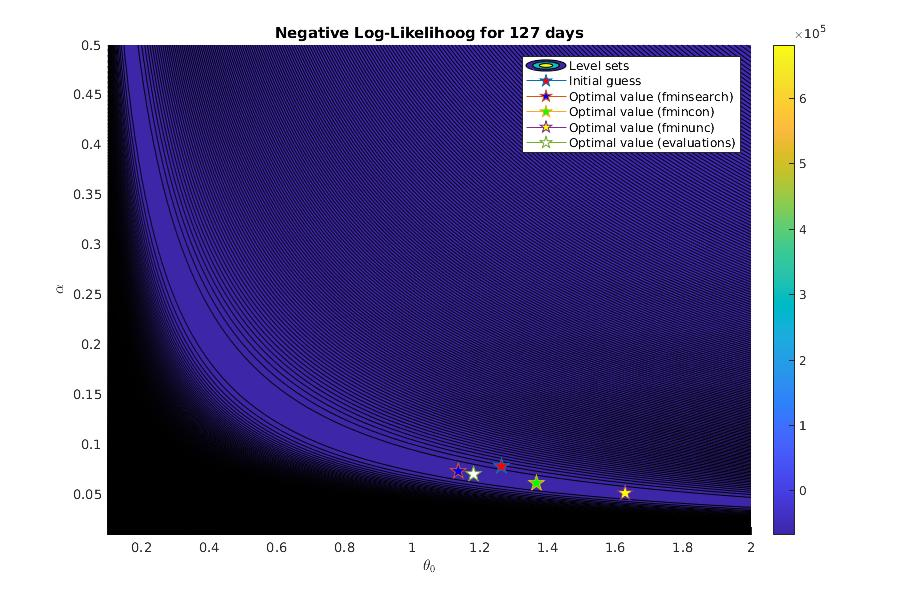
\includegraphics[width=0.5\textwidth]{../../MATLAB_Files/Results/likelihood/normal/Log-Likelihood.jpg}
\caption{Negative Log-Likelihood {\color{red}[Low quality picture]}.}
\label{fig:neg-LL}
\end{figure}
On Figure (\ref{fig:neg-LL}), we can see the level sets for the negative log-likelihood. The thick violet band is the region where the function reaches its minimums.\\
We can see the \textbf{initial guess} point, the result of three different \textbf{optimization tools} from MATLAB, and the minimum point that we found from the \textbf{evaluations} that generate the plot.
\begin{table}[]
\centering
\begin{tabular}{lccc}
\toprule
 & $\theta_0$ & $\alpha$ & $\theta_0\alpha$\\
 \midrule
 Initial guess & 1.629 & 0.060 & 0.098 \\
 fminsearch & 1.135 & 0.073 & 0.083 \\
 fmincon & 1.366 & 0.061 & 0.083 \\
 fminunc & 1.628 & 0.051 & 0.083 \\
 evaluations & 1.180 & 0.070 & 0.083 \\
 \bottomrule
\end{tabular}
\end{table}

\subsection{Calibration of the approximate negative log-likelihood in the $Z-$space}

We plot the Negative Log-Likelihood as a function of the parameters. The plots can be seen in Figure (\ref{fig:neg-LL}). We used all the training data (127 days of data) to construct and optimize the Negative Log-Likelihood.

\begin{figure}[H]
\centering
\includegraphics[width=0.5\textwidth]{../../MATLAB_Files/Results/likelihood/lamperti/Log-Likelihood.eps}
\caption{Negative Log-Likelihood {\color{red}[Low quality picture]}.}
\label{fig:neg-LLL}
\end{figure}
In Figure (\ref{fig:neg-LLL}), we can see the numerical level sets of the error function $\Psi$.\\
The center deep green band is the set $\mathbb{A}$ such that $\Psi(\mathbb{A})\in[0.05,0.1]$. We do not achieve relative error smaller than 0.05.\\
We observe a particular behavior over the curves $\theta_0\alpha=k\in\R^+$. However, it can be a numeric effect.\\
We also observe that: $$\mathbb{A}\cap\{(\theta_0,\alpha):\theta_0\alpha=0.083\}\neq\emptyset.$$
On the right, we observe some possible candidates for fixed points, that also satisfies the empirical condition $\theta_0\alpha=0.038$ from the error SDE.\\
We choose $(\theta_0,\alpha)=(2.200,0.038)$.\\
We interpret the set $\mathbb{A}$ as "the points where the transformation of the data, does not interfere with MLE".



\subsection{Model comparison} \label{Model_Comp}

We compare two candidate models to find the best-fit that maximizes the retained information,
\begin{itemize}
  \item Model 1: This model does not feature derivative tracking.
\begin{equation}
  \left\{
  \begin{array}{@{}rl@{}}
    dX_t \!\!\!&=  - \theta_0 (X_t - p_t) dt +\sqrt{2 \alpha \theta_0 X_t (1 - X_t)} dW_t\,, \quad t \in [0,T]  \\
   X_0  \!\!\!&=  x_0\in [0,1] \,,
 \end{array}\right.  \label{Model1}
\end{equation}
 with $\theta_0 > 0, \, \alpha > 0$.

%  \item Model 1: This model features derivative tracking, i.e. it is equivalent to (\ref{model:derivative_tracking_X}) with a diffusion term that is forecast dependent by including the term $p_t(1-p_t)$.
%  \begin{equation}
%  \begin{split}
%  dV_t &=  - \theta_t V_t \  dt + \sqrt{2 \theta_t \alpha p_t(1-p_t)(V_t +p_t ) (1-V_t-p_t)} \  dW_t  \\ %\quad t > 0
%  V_0 & = v_0
%  \end{split}\label{M2}
%  \end{equation}
%  with $\theta_t$ given by (\ref{theta_t}). This model has been used by [ insert ref ] and [ insert ref ]. Initial interest in this model stems from interest in long-term stationary solution, which may exists  if the forecast is constant. However, this is almost never occurs and thus including the term $p_t(1-p_t)$ is irrelevant. Additionally, the term $p_t(1-p_t)$ leads the model to become deterministic when the forecast is at the boundaries (i.e.$p=1$ or $p=0$)  which is not realistic. We have run computations on this model and the results were not satisfactory. Therefore, we exclude this model from further discussions.
%  

  \item Model 2: This model features derivative tracking and time-varying mean-reversion parameter:  
%i.e. it is equivalent to (\ref{model:derivative_tracking_X}).
%  \begin{align}
%  dV_t &=  - \theta_t V_t \  dt + \sqrt{2 \theta_t \alpha (V_t +p_t ) (1-V_t-p_t)} \  dW_t   \nonumber \\ %\quad t > 0
%  V_0 & = v_0 \,, \label{M2}
%  \end{align}
%  with $\theta_t$ given by (\ref{theta_t}).
\begin{equation}
  \left\{
  \begin{array}{@{}rl@{}}
    dX_t \!\!\!&= \big(\dot{p}_t  - \theta_t (X_t - p_t) \big) dt +\sqrt{2 \alpha \theta_0 X_t (1 - X_t)} dW_t\,, \quad t \in [0,T]  \\
   X_0  \!\!\!&=  x_0\in [0,1] \,,
 \end{array}\right.  \label{Model2}
\end{equation}
 with $\theta_0 > 0, \, \alpha > 0$ and .
\end{itemize}

\begin{table}[H]
\centering
\begin{tabular}{cccccc}
\toprule
Model & Forecast Provider & Method & Product $\theta_0\alpha$   & AIC & BIC \\ \midrule
Model 1 & Provider A & Gaussian Proxy & 0.105 & -58226 & -58211 \\
 &  & Shoji-Ozaki & 0.104 & -58226 & -58211 \\
 &  & Beta Proxy & 0.104 & -58286 & -58271 \\
 & Provider B & Gaussian Proxy & 0.105 & -58226   & -58211 \\
 &  & Shoji-Ozaki & 0.104 & -58226 & -58211 \\
 &  & Beta Proxy & 0.104 & -58288 & -58273 \\
 & Provider C & Gaussian Proxy & 0.105 & -58226 & -58211 \\
 &  & Shoji-Ozaki & 0.104 & -58226 & -58211 \\
 &  & Beta Proxy & 0.104 & -58286 & -58271 \\
Model 2 & Provider A & Beta Proxy & 0.097 & -73700   & -73685 \\ 
 & Provider B & Beta Proxy & 0.098 &  -73502 & -73487 \\ 
 & Provider C & Beta Proxy & 0.108 & -72518 & -72503 \\ 
\bottomrule
\end{tabular}
\caption{We compare the different models based on information criterion. \add }
\label{tab:model_comparison}
\end{table}


\subsection{Forecast providers comparison} \label{Forecast_Comp}
We compare forecasts from two different companies for the same period.
\begin{table}[H]
\centering
\begin{tabular}{ccc}
\toprule
Forecast Provider & Parameters $(\theta_0, \alpha)$ & Product $\theta_0\alpha$ \\ \midrule
Provider A  & $(1.930,0.050)$  &  0.097 \\
Provider B  & $(1.420,0.069) $  &  0.098 \\ 
Provider C  & $(1.380,0.078) $  &  0.108 \\ 
\bottomrule
\end{tabular}
\caption{Optimal parameters for different providers using Model 2 with Beta proxies.}
\label{tab:forcast_comparison}
\end{table}

{\color{red} Discuss to which extent it is needed more accuracy in the estimation of $\bm{\theta}$. How much data do we need to achieve enough accuracy for the estimates of the two parameters? Generally, such accuracy is application dependent.}

\subsection{Calibration of Model 2 with additional parameter $\delta$ TO DO}


After calibrating Model 2 on the training set, we can generate simulations of the wind power production for the time horizon of interest. The next Figure \ref{fig:simulation_paths} shows five simulated paths of the wind power production for each day of interest, assuming Model 2 specification and a given forecaster.

\begin{figure}[H]
\centering
\includegraphics[width=0.18\textwidth]{../../MATLAB_Files/Results/paths_testing_days/optimal_value/1.eps}
\includegraphics[width=0.18\textwidth]{../../MATLAB_Files/Results/paths_testing_days/optimal_value/2.eps}\\
\quad\\
\includegraphics[width=0.18\textwidth]{../../MATLAB_Files/Results/paths_testing_days/optimal_value/3.eps}
\includegraphics[width=0.18\textwidth]{../../MATLAB_Files/Results/paths_testing_days/optimal_value/4.eps}
\caption{Five simulated wind power production paths using the approximate MLEs for Model 2 $(\theta_0, \alpha ,\delta)=(1.2,0.1,0.6)$. }
\label{fig:simulation_paths}
\end{figure}

On the basis of the approximate MLEs for Model 2, we can obtain empirical pointwise confidence bands for the wind power production. The next Figure \ref{fig:confidence_bands} shows the empirical pointwise confidence bands for the wind power production for each day of interest, assuming Model 2 specification and a given forecaster.

\begin{figure}[H]
\centering
\includegraphics[width=0.35\textwidth]{../../MATLAB_Files/Results/bands_testing_days/optimal_value/1.eps}
\includegraphics[width=0.35\textwidth]{../../MATLAB_Files/Results/bands_testing_days/optimal_value/2.eps}\\
\quad\\
\includegraphics[width=0.35\textwidth]{../../MATLAB_Files/Results/bands_testing_days/optimal_value/3.eps}
\includegraphics[width=0.35\textwidth]{../../MATLAB_Files/Results/bands_testing_days/optimal_value/4.eps}
\caption{Empirical pointwise confidence bands for the wind power production using the approximate MLEs for Model 2 $(\theta_0, \alpha ,\delta)=(1.2,0.1,0.6)$. Blue line: real production.}
\label{fig:confidence_bands}
\end{figure}

\begin{figure}[ht!]
\centering
\includegraphics[width=0.48\textwidth]{../../MATLAB_Files/Results/histograms/classic/Optimal.eps}
\includegraphics[width=0.48\textwidth]{../../MATLAB_Files/Results/histograms/classic/Lamperti_Optimal.eps}
\end{figure}

We can see two histograms for the error transitions. On the left, using $(\theta_0^E,\alpha^E)$, while on the right, using $(\theta_0^L,\alpha^L)$.

%---END SECTION 6---

%---BEGIN SECTION 7---
\section{Conclusions} \label{Section_7}

We have proposed a method to produce stochastic wind power forecasts based on parametric SDEs. This method is agnostic of the wind power forecasting technology. Using this method, we were able to simulate future wind power production paths and obtain confidence bands. We conclude that Model 2 is a best-fit model. It features time-derivative tracking of the forecast, time-dependent mean reversion parameter, and a more natural diffusion term. Moreover, the model preserves the asymmetry of wind power forecast errors and their correlation structure.

We were also able to compare two different forecast providers with respect to their real-world performance on the aggregated data set and on specific wind farm sites. Finally, the model paves the way for stochastic optimal control methods enabling optimal decision making under uncertainty.
%---END SECTION 7---

%---BEGIN APPENDIX---
\section{Appendix} \label{Appendix}

\subsection{The model}
For a time horizon $T>0$ and  a parameter $\alpha > 0$ and $(\theta_t)_{t\in[0,T]}$ a positive deterministic  function,  let us consider the model  given by
\begin{equation}
  \left\{
  \begin{array}{@{}rl@{}}
    dX_t \!\!\!&= \big(\dot p_t - \theta_t (X_t-p_t)  \big)dt  +\sqrt{2 \alpha \theta_0 X_t (1-X_t)} dW_t\,, \quad t\in[0,T] \\
   X_0  \!\!\!&=  x_0\in [0,1] \,,
 \end{array}\right.  \label{eq:model}
\end{equation}
where $(p_t)_{t\in[0,T]}$ denotes the prediction function that satisfies $0\le p_t\le 1$ for all $t\in[0,T]$. This prediction function is assumed to be a smooth function of the time so that 
$$\sup_{t\in[0,T]}\bigl( |p_s| + |\dot p_s|\big) <+\infty .$$
The following proofs are based on standard arguments for stochastic processes that can be found e.g. in \cite{Alf} and \cite{KarShr} that we adapted to the setting of our model \eqref{eq:model}.
\begin{Thm}\label{thm:exun}
Assume that    
\begin{equation}\label{Assumption:1}
\forall  t\in[0,T],\;\; 0\le \dot p_t +\theta_tp_t\le \theta_t, \;\;\mbox{ and }\;\;
\sup_{t\in[0,T]}|\theta_t|<+\infty\tag{A}. 
\end{equation}
Then, there is a unique strong solution to \eqref{eq:model} s.t.  for all $t\in[0,T]$, $X_t\in[0,1]$ a.s.
\end{Thm}
\begin{proof}
Let us first consider the following SDE for $t\in[0,T]$
\begin{equation}\label{eq:eds1}
X_t=x_0+  \int_0^t\big(\dot p_s - \theta_s(X_s-p_s)  \big)ds  + \int_0^t\sqrt{2\alpha \theta_0 |X_s(1-X_s)|} dW_s, \quad x_0>0.
\end{equation}
According to Proposition 2.13, p.291 of \cite{KarShr}, under assumption  \eqref{Assumption:1} there is a unique strong solution $X$ to \eqref{eq:eds1}. Moreover, as the diffusion coefficient is of linear growth, we have  for all $p>0$ 
\begin{equation}\label{prop:fm}
\mathbb E[ \sup_{t\in[0,T]}|X_t|^p]<\infty.
\end{equation}
Then, it remains to show that for all $t\in[0,T]$, $X_t\in[0,1]$ a.s. For this aim, we need to use the so-called Yamada function $\psi_n$ that is a $\mathcal C^2$ function that satisfies a bench of useful properties:
\begin{align*}
&|\psi_n(x)|\underset{n\rightarrow+\infty}{\rightarrow}|x|, \;\; x{\psi'}_n(x)\underset{n\rightarrow+\infty}{\rightarrow}|x|, \;\; |\psi_n(x)|\wedge |x{\psi'}_n(x)| \le |x|\\
&{\psi'}_n(x)\le 1, \;\; \mbox{ and } {\psi''}_n(x)=g_n(|x|)\ge 0\;\; \mbox{ with } \;\; g_n(x)x\le \frac 2n\;\;  \mbox{ for all } x\in \mathbb R .
\end{align*}
See the proof of Proposition 2.13, p. 291 of \cite{KarShr} for the construction of such function.
Applying Itô's formula we get
\begin{align*}
\psi_n(X_t)&=\psi_n(x_0) +\int_0^t {\psi'}_n(X_s)(\dot p_s + \theta_s p_s - \theta_sX_s  \big)ds \\
&+ \int_0^t{\psi'}_n(X_s)\sqrt{2\alpha \theta_0 |X_s(1-X_s)|} dW_s + \alpha \theta_0 \int_0^t  g_n(|X_s|) |X_s(1-X_s)|ds.
\end{align*}
Now, thanks to  \eqref{Assumption:1}, \eqref{prop:fm} and to the above properties of $\psi_n$ and $g_n$, we get
$$
\mathbb E[\psi_n(X_t)]\le \psi_n(x_0) +\int_0^t \big(\dot p_s + \theta_sp_s -  \theta_s \mathbb E[{\psi'}_n(X_s)X_s] \big)ds + \frac{2\alpha  \theta_0}{n}\int_0^t \mathbb E |1-X_s|ds.
$$
Therefore, letting $n$ tends to infinity we use Lebesgue's theorem to get
$$
\mathbb E[|X_t|]\le x_0 +\int_0^t \big(\dot p_s + \theta_sp_s -  \theta_s \mathbb E|X_s| \big)ds.
$$
Besides, taking the expectation of \eqref{eq:eds1}, we get
$$
\mathbb E X_t=x_0+  \int_0^t\big(\dot p_s +\theta_sp_s - \theta_s \mathbb EX_s  \big)ds
$$
and thus we have 
$$
\mathbb E[|X_t| -X_t ]\le \int_0^t \theta_s \mathbb E[ X_s - |X_s| ]ds.
$$
Then, Gronwall's lemma gives us $\mathbb E[|X_t|]=\mathbb E X_t$ and thus for any $t\in[0,T]$ $X_t\ge0$ a.s. The same arguments work to prove that  for any $t\in[0,T]$ $Y_t:=1-X_t\ge0$  a.s.  since the process $(Y_t)_{t\in[0,T]}$ is solution to 
$$
dY_t= \big( \theta_t(1-p_t) -\dot p_t - \theta_tY_t  \big)dt  -\sqrt{2\alpha \theta_tY_t(1-Y_t)} dW_t,
$$
Then similarly, we need to assume that $\dot p_t +\theta_tp_t\ge 0$. This completes the proof.
\end{proof}

\begin{Thm}\label{thm:mod2}
Assume that assumptions of Theorem \ref{thm:exun} hold with $x_0\in]0,1[$.
Let $\tau_0:=\inf \{t\in[0,T],\; X_t=0\}$ and  $\tau_1:=\inf \{t\in[0,T],\; X_t=1\}$ with the convention that $\inf\emptyset=+\infty$. Assume in addition that for all $t\in[0,T]$,  $p_t\in]0,1[$ and that
\red{
\begin{equation}\label{Assumption:3}
\theta_t\geq \max\left(\frac{\alpha\theta_0+\dot p_t}{1-p_t},\frac{\alpha\theta_0-\dot p_t}{p_t}\right)\tag{B}. 
\end{equation}
}
 Then, $\tau_0=\tau_1=+\infty$ a.s.
\end{Thm}

\begin{proof}
For $t\in[0,\tau_0[$, we have 
$$
\frac{dX_t}{X_t}= \left(\frac{\dot p_t +\theta_t p_t}{X_t} - \theta_t\right)dt  +\sqrt{\frac{2\alpha \red{\theta_0}(1-X_t)}{X_t}} dW_t 
$$  
so that
$$
X_t=x_0\exp\Big(\int_0^t \frac{\dot p_s +\theta_sp_s- \red{\theta_0}\alpha}{X_s}ds+\alpha\red{\theta_0}t-  \int_0^t\theta_sds + M_t\Big),
$$
where $M_t=\int_0^t\sqrt{\frac{2\alpha \theta_0 (1-X_s)}{X_s}} dW_s$ is a continuous martingale. Then as for all $t\in[0,T]$, we have $\dot p_t +\theta_tp_t- \red{\theta_0}\alpha\ge0$, we deduce that
$$
X_t\ge x_0\exp\Big(\alpha\red{\theta_0}t-  \int_0^t\theta_sds + M_t\Big).
$$
By way of contradiction let us assume that  $\{\tau_0<\infty\}$, then letting $t\to \tau_0$ we deduce that $\lim_{t\to \infty} \mathbf 1_{\{\tau_0<\infty\}}M_{t\wedge \tau_0}=\mathbf -1_{\{\tau_0<\infty\}}\infty$ a.s. This leads to a contradiction since we know that continuous martingales likewise the Brownian motion cannot converge  almost surely to $+\infty$ or $-\infty$. It follows that $\tau_0=\infty$ almost surely. Next, recalling that  the process $(Y_t)_{t\geq 0}$  given by $Y_t=1-X_t$ is solution to 
$$
dY_t= \big( \theta_t(1-p_t) -\dot p_t - \theta_tY_t  \big)dt  -\sqrt{2\alpha \red{\theta_0}Y_t(1-Y_t)} dW_t 
$$
we deduce using similar arguments as above 
$\tau_1=\infty$ a.s. provided that $\theta_t(1-p_t) -\dot p_t -\alpha \red{\theta_0}\ge 0$.
 \end{proof} 

Remark: As the diffusion coefficient of $X$  given by  $x \mapsto \sqrt{2 \alpha \theta_0 x(1-x)}$  is strictly positive for all $x \in  ]0,1[$, the condition \eqref{Assumption:3}  ensures that the transformation between $Z$ and $X$ is bijective, so that we deduce the properties of existence and uniqueness of $Z$ from those of $X$. The application of  It\^{o}'s formula in Section \ref{Section_4} is subjected to the condition \eqref{Assumption:3} that avoids the process $X$ hits the boundaries of the interval $ ]0,1[$, otherwise the Lamperti transform is not applicable. 

%---END APPENDIX---

%---REFERENCES---

\nocite{*}
 
%\printbibliography
\printbibliography[keyword={Wind-SDE},title={References}]

\end{document}